\documentclass[a4paper]{jpconf}
\usepackage{graphicx}
\usepackage{hyperref}
%\usepackage{subcaption}

\newcommand{\GeV}{\ensuremath{\mathrm{\:GeV}}}
\newcommand{\TeV}{\ensuremath{\mathrm{\:TeV}}}
\newcommand{\pythia}{\texttt{Pythia8}}
\newcommand{\herwig}{\texttt{Herwig7}}
\newcommand{\chhh}{\ensuremath{\kappa_{\lambda}}}


\begin{document}

\title{Trilinear Higgs boson coupling variations for di-Higgs production with full NLO QCD predictions in \texttt{Powheg}}

\author{G.~Heinrich$^1$, S.~Jones$^2$, M.~Kerner$^3$, G.~Luisoni$^1$ and L.~Scyboz$^1$}

\address{$^1$ Max-Planck-Institut f\"ur Physik, F\"ohringer Ring 6, 80805 M\"unchen, Germany}
\address{$^2$ Theoretical Physics Department, CERN, Geneva, Switzerland}
\address{$^3$ Physik-Institut, Universit\"at Z\"urich, Winterthurerstrasse 190, 8057 Z\"urich, Switzerland}
\ead{gudrun@mpp.mpg.de, s.jones@cern.ch, mkerner@physik.uzh.ch, luisonig@gmail.com, scyboz@mpp.mpg.de}


\begin{abstract}
The Higgs couplings to other particles are increasingly well-measured by the ATLAS and CMS experiments. Yet there is still room for improvement in the limits set on the Higgs trilinear self-coupling $\lambda$, mainly due to the low cross-section for Higgs boson pair production. We present inclusive and differential results for the NLO QCD corrections to Higgs pair production with the full top-quark mass dependence, where the Higgs trilinear self-coupling is varied to non-SM values. The calculation of the two-loop virtual contributions has been performed numerically using CPUs and GPUs. The fixed-order calculation is supplemented by parton showering within the \texttt{Powheg-BOX-V2} event generator, and both \pythia~and \herwig~parton-shower algorithms are implemented in a preliminary study of shower effects.
\end{abstract}


\section{Introduction}

Impressive experimental constraints have been set on the Higgs boson couplings to vector bosons and heavy fermions. The Higgs potential, in contrast, leaves more room for New Physics. The Higgs boson trilinear self-coupling $\lambda$ can be constrained directly by exclusion limits on Higgs pair production $pp \to hh$.
%The best experimental limit is given by ATLAS with $-5.0 < \kappa_{\lambda} < 12.1$ at $95\%$ confidence level~\cite{ATLAS-CONF-2018-043}, from a combination of $hh \to b\bar{b}b\bar{b}, b\bar{b}\tau^+ \tau^-$ and $b\bar{b}\gamma\gamma$ channels.
Higher-order corrections to Higgs pair production are routinely calculated in the heavy top-quark mass limit (HTL) $m_t \to \infty$, where the top-quark degrees of freedom are integrated out. The NLO QCD corrections with the full top-quark mass dependence were only computed more recently~\cite{Borowka:2016ehy,Borowka:2016ypz,Baglio:2018lrj}. Based on a numerical evaluation of the two-loop contribution to $gg \to hh$ performed via sector decomposition, results were computed at NLO QCD with full top-quark mass dependence for a class of extensions of the SM in Ref.~\cite{Buchalla:2018yce}. 

In the following, an implementation of the full NLO QCD corrections into the \texttt{Powheg-BOX-V2} event generator~\cite{Nason:2004rx,Frixione:2007vw,Alioli:2010xd} is presented. In this framework, the Higgs trilinear self-coupling can be varied, as well as the top-Higgs Yukawa coupling. Total cross-sections are computed for $\sqrt{s}=13,14$ and $27 \TeV$ at the (HE-)LHC. Differential results are shown for $\sqrt{s}=14 \TeV$. The fixed-order calculation is then matched to both $\pythia$~\cite{Sjostrand:2014zea} and $\herwig$~\cite{Bellm:2017bvx} parton showers. For a more detailed description, the reader is referred to Ref.~\cite{Heinrich:2019bkc}.

\section{Description of the calculation}

The calculation is based on the setup presented in Ref.~\cite{Heinrich:2017kxx} for the case of the SM. The leading-order amplitude has been computed analytically. The real-emission contributions were implemented in \textsc{GoSam}~\cite{Cullen:2011ac,Cullen:2014yla} and interfaced to the \texttt{Powheg-BOX}, and the corresponding scalar one-loop amplitudes were evaluated with \texttt{Ninja}~\cite{Peraro:2014cba}, \texttt{golem95C}~\cite{Binoth:2008uq,Cullen:2011kv} and \texttt{OneLOop}~\cite{vanHameren:2010cp} (except for the scalar four-point function, which is taken from \texttt{VBFNLO}~\cite{Arnold:2008rz,Baglio:2014uba} for numerical stability reasons).
The two-loop amplitude for the full-theory virtual contribution was adapted from Refs.~\cite{Borowka:2016ehy,Borowka:2016ypz}, which used an extension of the \textsc{GoSam} package. There, the integral reduction was performed with \textsc{Reduze2}~\cite{vonManteuffel:2012np}, and the integrals were numerically evaluated with \textsc{SecDec3}~\cite{Borowka:2015mxa}. For a fast convergence, the integration was performed within a Quasi-Monte-Carlo implementation using a rank-1 shifted lattice~\cite{Borowka:2018goh,Jones:2016bci}. The integrals were computed with 16 dual \textsc{NVidia Tesla K20Xm} GPUs. The top-quark and Higgs masses have been set to $m_t=173 \GeV$ and $m_h = 125 \GeV$. Thus, the integrals depend only on the two Mandelstam invariants $\hat{s}$ and $\hat{t}$.

A grid for the two-loop amplitude was constructed in both variables using $5291$ pre-sampled phase-space points. %The trilinear Higgs self-coupling enters the full amplitude through the contribution of triangle-like diagrams $\mathcal{M}_T$, as the one shown at leading order in Fig.~\ref{}.
We split the amplitude in two contributions: diagrams containing the trilinear Higgs coupling are called \textit{triangle-like}, and those that do not \textit{box-like} (see Fig.~\ref{fig:lodiagrams} for two leading-order diagrams). 


\begin{figure}[htb!]
\begin{minipage}[(a)]{0.5\textwidth}
\centering
\includegraphics[width=0.6\textwidth]{figures/{hh1}.eps}
\end{minipage}
\quad
\begin{minipage}[(a)]{0.5\textwidth}
\centering
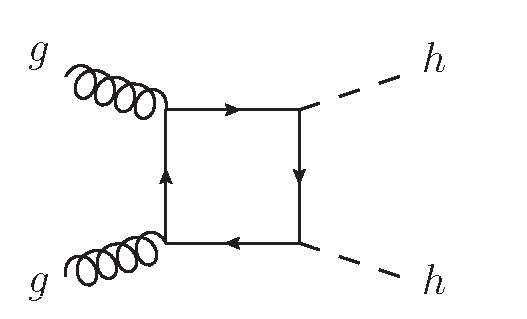
\includegraphics[width=0.6\textwidth]{figures/hh2.eps}
\end{minipage}
\caption{Triangle-like (left) and box-like (right) diagrams contribute to the full amplitude. The former contain the Higgs self-coupling, while the latter do not. \label{fig:lodiagrams}}
\end{figure}


At any order in QCD, the squared matrix-element can thus be written as a second-order polynomial in $\lambda$:

\begin{equation}
M_{\lambda} \equiv |{\cal M}_\lambda|^2=\mathcal{M}_B^* \mathcal{M}_B + \lambda \left( \mathcal{M}_B^* \mathcal{M}_T + \mathcal{M}_T^* \mathcal{M}_B  \right) +  \lambda^2 \mathcal{M}_T^* \mathcal{M}_T \;.
\label{eq:2ndorder}
\end{equation}

The two-loop amplitude for an arbitrary value of $\lambda$ can be reconstructed from the squared matrix-element computed for three different values of $\lambda$. In our case, we chose $\chhh=\lambda_{\mathrm{BSM}}/\lambda_{\mathrm{SM}} \in \lbrace -1, 0, 1 \rbrace$ and generate a new grid for the user-defined value of $\lambda$, where the amplitude for each pre-sampled phase-space point is calculated as:
	
\begin{equation}
M_{\lambda} =M_0\cdot(1-\lambda^2)+\frac{M_1}{2}\cdot(\lambda+\lambda^2) + \frac{M_{-1}}{2}\cdot(-\lambda+\lambda^2)\;.
\end{equation}

An interpolation framework takes the produced grid as input and the amplitude at \textit{any} phase-space point $M_{\lambda}(\hat{s}, \hat{t})$ can be interfaced to \texttt{Powheg}.



\section{Total and differential cross-sections for variations of the trilinear coupling}

The results given below are produced using the PDF4LHC15\_nlo\_30\_pdfas sets~\cite{Butterworth:2015oua,CT14,MMHT14,NNPDF} interfaced to \texttt{Powheg} via \texttt{LHAPDF6}~\cite{Buckley:2014ana}, with the corresponding value of $\alpha_s$. The top-quark mass is renormalised in the on-shell scheme and is set to $m_t=173 \GeV$, as in the virtual amplitude. The mass of the Higgs boson is fixed to $m_h=125 \GeV$, and the top-quark and Higgs widths are set to zero. Jets are clustered using the anti-$k_T$ algorithm~\cite{Cacciari:2008gp} as implemented in \texttt{FastJet}~\cite{Cacciari:2005hq, Cacciari:2011ma}, with a jet distance parameter of $R=0.4$ and a minimum transverse momentum requirement of $p_{T} = 20 \GeV$. The central renormalisation and factorisation scales are set to $\mu_R = \mu_F = \mu_0 = m_{hh} / 2$. Scale uncertainties are estimated by 2-point variations $\mu_R = \mu_F = c\, \mu_0$, with $c \in \lbrace {0.5, 2.0} \rbrace$.

Total cross-sections for Higgs pair production at the (HE-)LHC are shown in Table~\ref{tab:sigmatot}, for centre-of-mass energies of $\sqrt{s}=13,14$ and $27 \TeV$ and different values of the Higgs self-coupling $\chhh = \lambda_{\mathrm{BSM}} / \lambda_{\mathrm{SM}}$. They are accompanied by their relative scale uncertainties, which are of the order $\mathcal{O}(10-20\%)$. Notably, the $K$-factors at $14 \TeV$ show a sizeable dependence on the trilinear coupling $\chhh$. In the HTL at NLO QCD, Ref.~\cite{Grober:2015cwa} suggested that the dependence of the $K$-factors on $\chhh$ are of the order $\mathcal{O}(2-3\%)$. In the full theory, the $K$-factors are found between $1.56$ and $2.15$ for variations of the trilinear coupling $-5 \leq \chhh \leq 12$, see Fig.~\ref{fig:Kfacvariation}. 

\begin{table}[htb!]
\begin{center}
%\setlength{\extrarowheight}{3.0pt}
\begin{tabular}{| c | c | c |c|c|}
%\Xhline{2\arrayrulewidth}
\hline
&&&&\\
$\lambda_{\mathrm{BSM}}/\lambda_{\mathrm{SM}}$ & $\sigma_{\rm{NLO}}@13 \mathrm{TeV}$\,[fb]& $\sigma_{\rm{NLO}}@14 \mathrm{TeV}$\,[fb] & $\sigma_{\rm{NLO}}@27 \mathrm{TeV}$\,[fb] &K-factor@14TeV\\
&&&&\\
\hline
-1& 116.71$^{+16.4\%}_{-14.3\%}$  & 136.91$^{+16.4\%}_{-13.9\%}$& 504.9$^{+14.1\%}_{-11.8\%}$ & 1.86 \\
\hline
0& 62.51$^{+15.8\%}_{-13.7\%}$ & 73.64$^{+15.4\%}_{-13.4\%}$& 275.29$^{+13.2\%}_{-11.3\%}$& 1.79  \\
\hline 
1& 27.84$^{+11.6\%}_{-12.9\%}$ & 32.88$^{+13.5\%}_{-12.5\%}$&127.7$^{+11.5\%}_{-10.4\%}$ &1.66\\
\hline
2 & 12.42$^{+13.1\%}_{-12.0\%}$ & 14.75$^{+12.0\%}_{-11.8\%}$ &  59.10$^{+10.2\%}_{-9.7\%}$ & 1.56 \\
\hline
2.4& 11.65$^{+13.9\%}_{-12.7\%}$ & 13.79$^{+13.5\%}_{-12.5\%}$& 53.67$^{+11.4\%}_{-10.3\%}$ & 1.65 \\
\hline
3& 16.28$^{+16.2\%}_{-15.3\%}$ & 19.07$^{+17.1\%}_{-14.1\%}$ & 69.84$^{+14.6\%}_{-12.1\%}$ & 1.90 \\
\hline 
5& 81.74$^{+20.0\%}_{-15.6\%}$  & 95.22$^{+19.7\%}_{-11.5\%}$& 330.61$^{+17.4\%}_{-13.6\%}$ & 2.14 \\
\hline 
\end{tabular}
\end{center}
\caption{Total cross-sections are given for Higgs pair production at NLO QCD at (HE-)LHC for centre-of-mass energies of $\sqrt{s}=13,14$ and $27 \TeV$. The scale uncertainties are given in percent.
\label{tab:sigmatot}}
\end{table}

\begin{figure}[htb!]
  \centering
    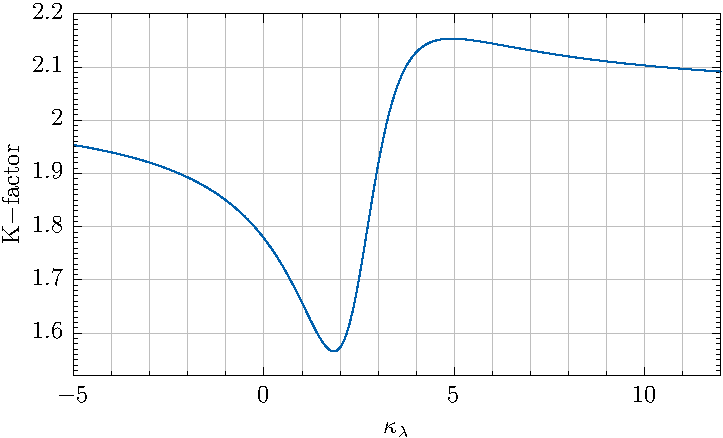
\includegraphics[width=0.65\textwidth]{figures/Kfactor.pdf}
%  \includegraphics[width=\textwidth]{figures/}
%    \caption{\label{fig:lambda_large_27}}
\caption{The dependence of the $K$-factor on the trilinear Higgs self-couplings $\chhh$ is given at $\sqrt{s}=14$\,TeV in the full theory.}
\label{fig:Kfacvariation}
\end{figure}

In Fig.~\ref{fig:lambdavar14TeV}, distributions of the invariant mass of the Higgs pair system $m_{hh}$ are displayed for different values of $\chhh$. They exhibit a characteristic dip around $m_{hh} \sim 350 \GeV$ for values of the trilinear coupling around $\chhh = 2.4$, which is not present in the SM case. This value of the trilinear self-coupling corresponds to a maximally destructive interference between triangle-like and box-like diagrams.


\begin{figure}[htb!]
\begin{minipage}[(a)]{0.5\textwidth}
\includegraphics[width=1.\textwidth]{figures/{NLO_cHHH_1_2_2.4_0_mHH-paper}.pdf}
\end{minipage}
\hfill
\begin{minipage}[(a)]{0.5\textwidth}
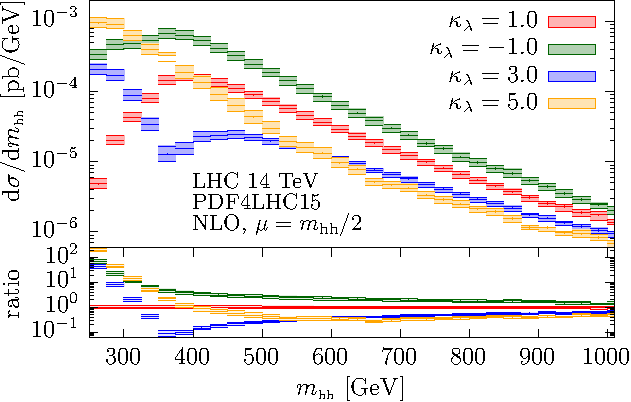
\includegraphics[width=1.\textwidth]{figures/NLO_cHHH_1_-1_3_5_mHH-paper.pdf}
\end{minipage}
\caption{Higgs boson pair invariant mass distributio	ns for various
  values of $\chhh$  at $\sqrt{s}=14$\,TeV. The uncertainty bands are from
  scale variations as described in the text.\label{fig:lambdavar14TeV}}
\end{figure}

Note that since the contributions can be separated in triangle- and box-like diagrams, the top-Higgs Yukawa coupling $y_t$ can easily be varied within the same code by rescaling the monomials in Eq.~(\ref{eq:2ndorder}):

\begin{equation}
|{\cal M}_\lambda|^2=y_t^4 \left[ \mathcal{M}_B^* \mathcal{M}_B + \frac{\chhh}{y_t} \left( \mathcal{M}_B^* \mathcal{M}_T + \mathcal{M}_T^* \mathcal{M}_B  \right) +  \left( \frac{\chhh}{y_t} \right)^2 \mathcal{M}_T^* \mathcal{M}_T \right] \;.
\end{equation}

For example, $\sigma(y_t=1.2,\chhh=1)=(1.2)^4\,\sigma(y_t=1,\chhh=1/1.2)$. Fig.~\ref{fig:ytvars}  shows the distribution of $m_{hh}$ for extreme values of the top-Higgs Yukawa coupling that are still not experimentally excluded.

\begin{figure}[htb!]
  \centering
    \includegraphics[width=0.65\textwidth]{figures/{NLO_CPP_yt_0.8_1.2_mHH}.pdf}
\caption{The distribution of the Higgs pair invariant mass $m_{hh}$ for values of the top-Higgs Yukawa coupling $y_t \in \lbrace 0.8, 1, 1.2 \rbrace$.}
\label{fig:ytvars}
\end{figure}

\section{Parton-shower matched results}

We now consider NLO distributions matched to a parton shower. The Les Houches Events (LHE)~\cite{Alwall:2006yp} files produced by \texttt{Powheg} are used as input to the \texttt{Pythia8.235} and \texttt{Herwig7.1.4} parton showers. In the case of \herwig, both the default angular-ordered $\tilde{q}$ and the dipole showers are compared. The radiation-regulating \texttt{hdamp} parameter in \texttt{Powheg} is set to $\texttt{hdamp}=250 \GeV$. Multiple-parton interactions and hadronisation are switched off. The default tunes are used for both parton showers.

%We compare the fixed-order NLO result to predictions matched to \pythia~(PP8) and the \herwig~$\tilde{q}-$ordered (PH7-$\tilde{q}$), respectively dipole (PH7-dipole) showers. 

Fig.~\ref{fig:lambdavar14TeV_pTHH_dRHH_showers} displays the transverse momentum of the Higgs boson pair $p_T^{hh}$ and the separation between the two Higgs bosons $\Delta R^{hh} = \sqrt{(\eta_1 - \eta_2)^2 + (\phi_1 - \phi_2)^2}$. Considering first the distribution of $p_T^{hh}$, both \herwig~parton showers (PH7-$\tilde{q}$ and PH7-dipole) generate similar results and reproduce the fixed-order NLO prediction in the far-$p_T^{hh}$ range. In contrast, \pythia~agrees with \herwig~only for small transverse momenta, while it produces much harder radiation in the tail of the distribution. The same comments apply to the $\Delta R^{hh}$ observable in the shower-dominated region $0 < \Delta R^{hh} < \pi$. Large parton-shower matching uncertainties in Higgs pair production have already been emphasized~\cite{Jones:2017giv}. 

\begin{figure}[htb!]
\begin{minipage}[(a)]{0.5\textwidth}
\includegraphics[width=1.\textwidth]{figures/{NLO_PP8_PH7_PH7D_cHHH_1_ptHH}.pdf}
\end{minipage}
\hfill
\begin{minipage}[(a)]{0.5\textwidth}
\includegraphics[width=1.\textwidth]{figures/{NLO_PP8_PH7_PH7D_cHHH_1_dRHH}.pdf}
\end{minipage}
\caption{The transverse momentum $p_T^{hh}$ of one (any) Higgs boson and the separation between the two Higgs bosons $\Delta R^{hh}$ are shown for the fixed-order NLO calculation and three parton showers, in 
the $\chhh=1$ case.\label{fig:lambdavar14TeV_pTHH_dRHH_showers}}
\end{figure}


\section{Conclusion}

We have presented a new package for Higgs boson pair production at NLO QCD with full top-quark mass dependence. In this package, the trilinear Higgs self-coupling can be varied explicitly. Within the same code, simultaneous variations of the top-Higgs Yukawa coupling can also be produced. The public code for the \texttt{Powheg-BOX-V2} event generator can be found at the website \href{http://powhegbox.mib.infn.it}{\tt http://powhegbox.mib.infn.it} in the {\tt User-Processes-V2/ggHH} subdirectory. As a side note, approximations related to the HTL can be enabled for comparison purposes. We have emphasized that the full $m_t$-dependent NLO QCD corrections are accompanied by large $K$-factors. Moreover, they induce a sizeable dependence of the $K$-factors on the trilinear Higgs self-coupling $\chhh$, which is not present in the HTL. We have compared fixed-order predictions at NLO QCD to parton-shower matched results. Both the \pythia~and \herwig~($\tilde{q}$ and dipole) parton showers can be matched directly to LHE files produced by \texttt{Powheg}. Full particle-level events can thus be produced with our framework, including Higgs boson decays and hadronisation.



\section*{References}

\bibliographystyle{iopart-num}
\bibliography{acat}{}

\end{document}


